%%%%%%%%%%%%%%%%%%%%%%%%%%%%%%%%%%%%%%%%%%%%%%%%%%%%%%%%%%%%%%%%%%%%%%
% Source: http://www.howtotex.com
%%%%%%%%%%%%%%%%%%%%%%%%%%%%%%%%%%%%%%%%%%%%%%%%%%%%%%%%%%%%%%%%%%%%%%
\documentclass[paper=a4, fontsize=11pt]{scrartcl}
\usepackage[T1]{fontenc}
\usepackage{fourier}

\usepackage{minted}

\usepackage[english]{babel}                                                                                                                     % English language/hyphenation
\usepackage[protrusion=true,expansion=true]{microtype}  
\usepackage{amsmath,amsfonts,amsthm} % Math packages
\newcommand*{\rttensor}[1]{\overline{\overline{#1}}}
\newcommand{\pfrac}[2]{\frac{\partial#1}{\partial#2}}

\usepackage[pdftex]{graphicx}  


\usepackage{url}
\usepackage{hyperref}


\usepackage[numbers]{natbib}
%\usepackage[style=ieee]{biblatex}

%%% Custom sectioning

\usepackage{sectsty}
\allsectionsfont{\centering \normalfont\scshape}


%%% Custom headers/footers (fancyhdr package)
\usepackage{fancyhdr}
\pagestyle{fancyplain}    
\fancyhead{}% No page header
\fancyfoot[L]{}% Empty 
\fancyfoot[C]{}% Empty
\fancyfoot[R]{\thepage}% Pagenumbering
\renewcommand{\headrulewidth}{0pt}% Remove header underlines
\renewcommand{\footrulewidth}{0pt}% Remove footer underlines
\setlength{\headheight}{10.6pt}


%%% Equation and float numbering
\numberwithin{equation}{section}                % Equationnumbering: section.eq#
\numberwithin{figure}{section}                  % Figurenumbering: section.fig#
\numberwithin{table}{section}                           % Tablenumbering: section.tab#


%%% Maketitle metadata
\newcommand{\horrule}[1]{\rule{\linewidth}{#1}}         % Horizontal rule

\title{%\vspace{-1in}      
    \usefont{OT1}{bch}{b}{n}
    \normalfont\normalsize \textsc{Kevin T. Crofton Department of Aerospace and Ocean Engineering} \\ [25pt]
    \horrule{0.5pt} \\[0.4cm]
    \huge Magneto Rayleigh-Taylor Instability for an Annulus using Finite Volume Method with the MagnetoHydroDynamic Equations  \\
    \horrule{2pt} \\[0.5cm]}
\author{\normalfont\normalsize
  Robert Masti\\[-3pt]  
  \normalsize\today}
\date{}


%%% Begin document
\begin{document}
\maketitle
\section{MRT Overview \& Simulation Setup}\label{sec:ovrvw}
The magneto Rayleigh-Taylor instability (MRT) occurs when there is a heavy fluid supported by a light fluid under the influence of gravity with the addition of magnetic fields. Depending on the orientation of these magnetic fields they can have stabilizing characteristics for the growth of this instability. MRT is a hydrodynamic instability so it can be modeled using the ideal MagnetoHydroDynamic (MHD) equations. This instability is one of the most detrimental instabilities in the plasma communities attempt to reach fusion ignition. Specifically as it applies to inertial confinement fusion devices such as the one at NIF in the Direct Drive concept shown in Figure~\ref{fig:ovrvw:dd} part (c). The densities, pressures, and acceleration are going to be taken from \href{https://www.astro.princeton.edu/~jstone/Athena/tests/rt/rt.html}{Athena Webpage} to at least get the simulation setup, and then transition to realistic densities, pressures, and acceleration.


  \begin{figure}[!htb]
    \centering
    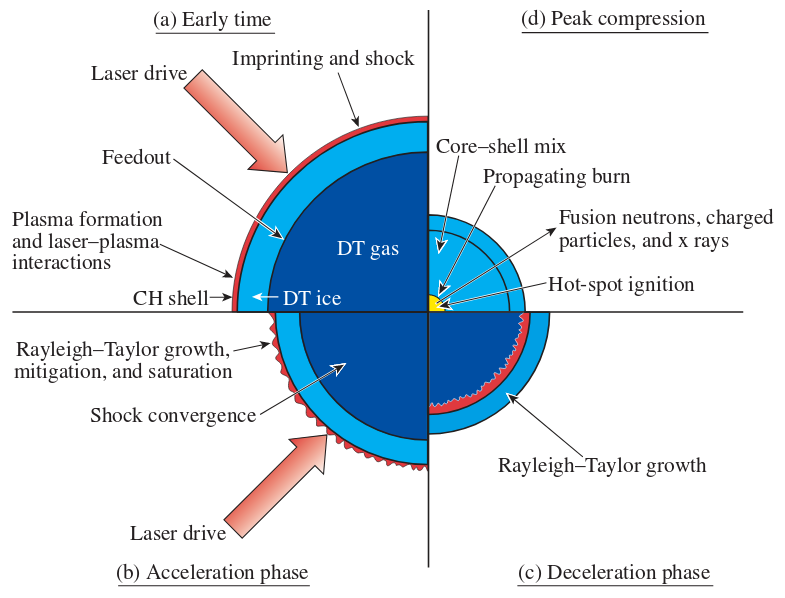
\includegraphics[width=0.9\linewidth]{fig/DDfusion}\label{fig:ovrvw:dd}
    \caption{Shows the four main stages during a typical direct-drive target implosion.\cite{craxton2015}}
  \end{figure}

\subsection{MHD Equation System}

The mhd equations allow for the incorporation of electric and magnetic fields as they influence a conducting medium. It has the continuity, conservation of momentum and energy like in Euler equation, but it has the addition of an induction equation for the magnetic field. For a plasma there is co existing electrons and ions, and in MHD the electron fluid equations are used to derive the electric field used in the induction equation, and the extent of this electric field can extend or retract the equation system. Initially just the lorentz force term will be used as the electric field contribution to the induction equation. Assuming ideal gas EOS the MHD equations are given by

\minipage{\textwidth}
  \minipage{0.48\textwidth}
  \begin{align*}
    \pfrac{\rho}{t} + \nabla \cdot \left[\rho \mathbf{u}\right] &= 0 \\
    \pfrac{\rho \mathbf{u}}{t} + \nabla \cdot \left[\rho \mathbf{u}\mathbf{u}^T - \mathbf{b}\mathbf{b}^T + \mathbb{I}\left(P + \frac{1}{2}|\mathbf{b}|^2\right)\right] &= 0 \\
    \pfrac{\epsilon}{t} + \nabla \cdot \left[\left(\epsilon + P + \frac{1}{2}|\mathbf{b}|^2\right)\mathbf{u}- \mathbf{b}\cdot\mathbf{u}\mathbf{b}\right] &= 0 \\
    \pfrac{\mathbf{b}}{t} + \nabla\times\mathbf{e} &= 0 \\
  \end{align*}
  \endminipage\hfill
  \minipage{0.48\textwidth}
  \begin{align*}
    \mathbf{b} &= \frac{\mathbf{B}}{\sqrt{\mu_0}} \\
    \mathbf{e} &= - \mathbf{u} \times \mathbf{b} +\left(\mathbf{e}^{external}\rightarrow\mathbf{0}\right)\\
    \epsilon &= \epsilon_{internal} + \frac{1}{2}\rho|\mathbf{u}|^2 + \frac{1}{2}|\mathbf{b}|^2\\
    P &=\rho \epsilon_{internal} (\gamma - 1) \\
  \end{align*}
  \endminipage\hfill
  \endminipage, where there is no external electric fields ($e.q.\;\eta \mathbf{j}$). The equation for the magnetic field must be manipulated with vector identities into a divergence form through
  \begin{align*}
    \pfrac{\mathbf{b}}{t} + \nabla\times(-\mathbf{u}\times\mathbf{b}) &= 0\\
    \pfrac{\mathbf{b}}{t} - \left[\mathbf{u}(\nabla\cdot\mathbf{b})-\mathbf{b}(\nabla\cdot\mathbf{u})+(\mathbf{b}\cdot \nabla)\mathbf{u}-(\mathbf{u}\cdot\nabla)\mathbf{b}\right] &= 0\\
    \pfrac{\mathbf{b}}{t} - \left[\nabla\cdot(\mathbf{b}\mathbf{u}^T)-\nabla\cdot(\mathbf{u}\mathbf{b}^T)\right] &= 0\\
    \pfrac{\mathbf{b}}{t} + \nabla\cdot\left[\mathbf{u}\mathbf{b}^T-\mathbf{b}\mathbf{u}^T\right] &= 0\\
  \end{align*}, and it now is in divergence form which can be used to write into the tensor product form. The conservative variable are density, momentum, total energy density, and magnetic field. For the given problem however it is more convenient to rewrite as
\begin{equation}\label{eqn:mhdvector}
  \pfrac{\mathbf{Q}}{t} + \nabla \cdot \rttensor{T} = 0
\end{equation}
where $\mathbf{Q}$ is the conserved variables vector, and $\rttensor{T}$ is the flux tensor. Where the conserved variables vector, and flux tensor, are given by
\[
  \mathbf{Q}=
  \begin{bmatrix}
    \rho  \\
    \rho \mathbf{u}  \\
    \epsilon\\
    \mathbf{b} 
  \end{bmatrix}
  ,\quad \rttensor{T} =
  \begin{bmatrix}
    \rho \mathbf{u}  \\
    \rho \mathbf{u}\mathbf{u}^T - \mathbf{b}\mathbf{b}^T + \mathbb{I}\left(P + \frac{1}{2}|\mathbf{b}|^2\right)\\
    \left(\epsilon + P + \frac{1}{2}|\mathbf{b}|^2\right)\mathbf{u}- \mathbf{b}\cdot\mathbf{u}\mathbf{b}\\
    \mathbf{u}\mathbf{b}^T-\mathbf{b}\mathbf{u}^T
  \end{bmatrix}
\]
, respectively. 

\subsection{Discretization \& Flux Formulation}
  \begin{figure}[!htb]
    \centering
    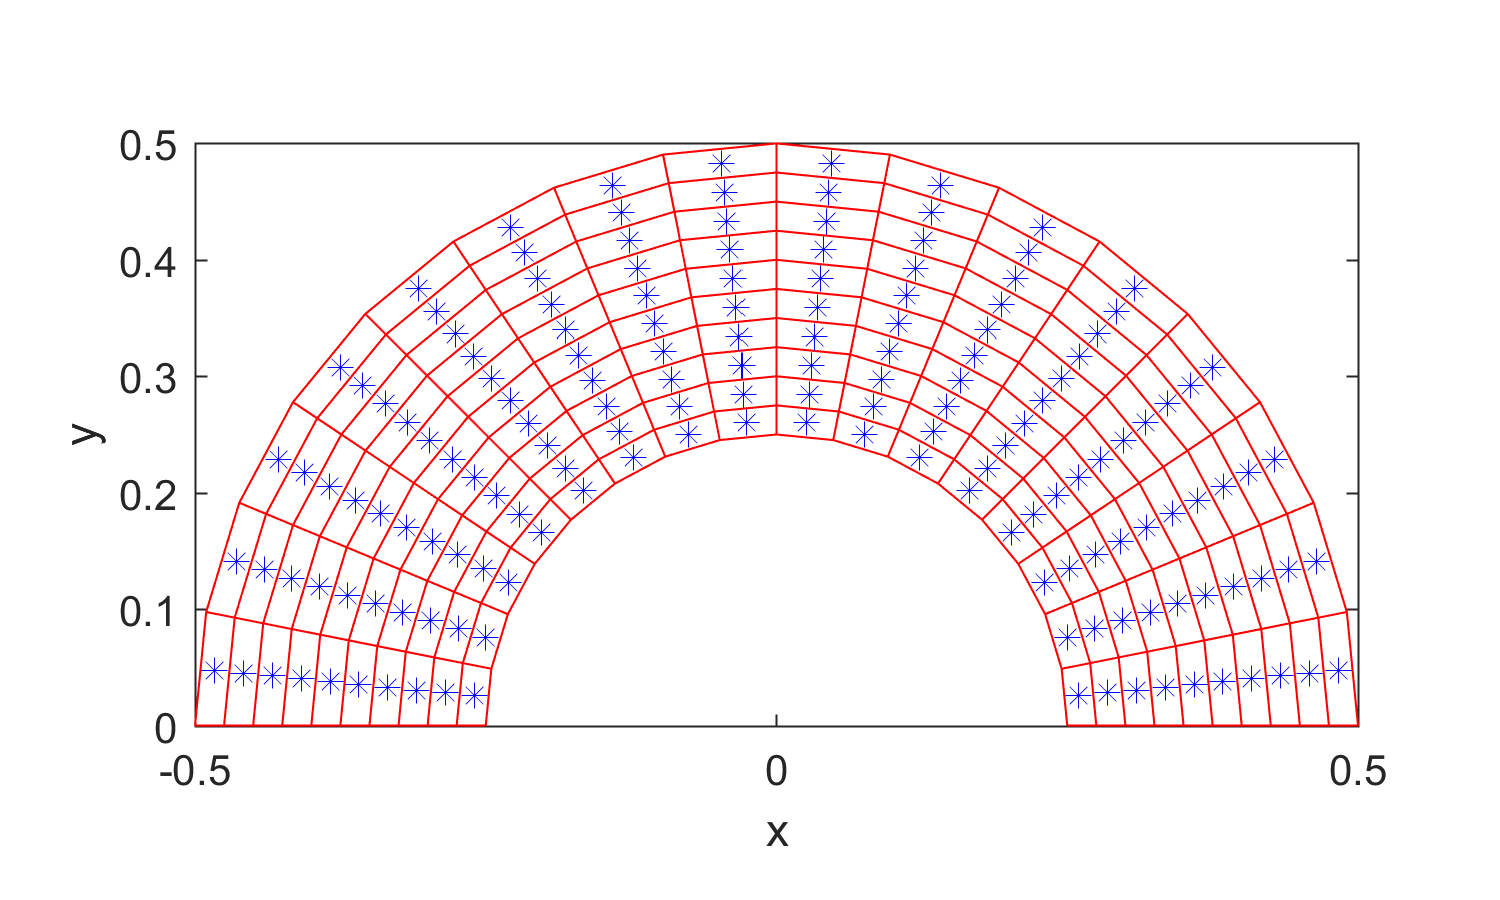
\includegraphics[width=0.8\linewidth]{fig/16x10mesh}\label{fig:ovrvw:mesh}
    \caption{A mesh example using 16 cells in the i direction and 10 cells in the j direction with cell centers highlighted}
  \end{figure}

The simulation setup will use a discretization shown in Figure~\ref{fig:ovrvw:mesh} where the coordinates are unitless currently. The mesh generation is done in matlab for this simplistic geometry. In order to evaluate the flux in the x and y direction the normal vectors on the cell faces are required. With the normal vectors and areas known the fluxes can be determined for MHD in curvilinear coordinates as

\begin{equation} \label{eqn:mhdvecflux}
  \pfrac{\mathbf{Q}}{t} + \pfrac{\mathbf{F}}{x} + \pfrac{\mathbf{G}}{y} = 0
\end{equation},
where $\mathbf{F}$ is the $\hat{x}$ direction flux, and $\mathbf{G}$ is the $\hat{y}$ direction flux. Expanding the flux tensor through evaluating the dyadic terms, and collecting non-zero unit vectors $\mathbf{F}$, and $\mathbf{G}$ can be easily found. Equation~\ref{eqn:mhdvecflux} can be expanded into for cartesian coordinates into

\[
  \pfrac{}{t}
  \begin{bmatrix}
    \rho  \\
    \rho u  \\
    \rho v \\
    \rho w \\
    \epsilon\\
    b_x \\
    b_y \\
    b_z 
  \end{bmatrix}
  \;+\;\pfrac{}{x}
  \begin{bmatrix}
    \rho u  \\
    \rho u^2 + P + \frac{1}{2}|\mathbf{b}|^2 - b_x^2\\
    \rho u v - b_x b_y \\
    \rho u w - b_x b_z \\
    \left(\epsilon+ P + \frac{1}{2}|\mathbf{b}|^2 \right) u - b_x \mathbf{u}\cdot\mathbf{b}\\
    0 \\
    b_y u - b_x v \\
    b_z u - b_x w 
  \end{bmatrix}
  \;+\;\pfrac{}{y}
  \begin{bmatrix}
    \rho v  \\
    \rho v u - b_y b_x\\
    \rho v^2 + P + \frac{1}{2}|\mathbf{b}|^2 - b_y^2\\
    \rho v w - b_y b_z \\
    \left(\epsilon+ P + \frac{1}{2}|\mathbf{b}|^2  \right) v - b_y\mathbf{u}\cdot\mathbf{b}\\
    b_x v - b_y u \\
    0 \\
    b_z v - b_y w 
  \end{bmatrix}
  =0
\]

For an arbitrarily oriented cell with interface normal $\hat{n} = n_x \hat{x} + n_y\hat{y}$ that maps to compuational grid $(i,j)\rightarrow(\eta,\xi)$) this form can be rewritten as

\[
  \pfrac{}{t}
  \begin{bmatrix}
    \rho  \\
    \rho u  \\
    \rho v \\
    \rho w \\
    \epsilon\\
    b_x \\
    b_y \\
    b_z 
  \end{bmatrix}
  \;+\;\pfrac{}{\eta}
  \begin{bmatrix}
    \rho c_*  \\
    \rho u c_* + P n_x + \frac{1}{2}|\mathbf{b}|^2 n_x- b_x b_*\\
    \rho v c_* + P n_y + \frac{1}{2}|\mathbf{b}|^2 n_y - b_y b_* \\
    \rho w c_* - b_z b_*\\
    \left(\epsilon+ P + \frac{1}{2}|\mathbf{b}|^2 \right) c_* - b_* \mathbf{u}\cdot\mathbf{b}\\
    b_x c_* - b_* u\\
    b_y c_* - b_* v \\
    b_z c_* - b_* w 
  \end{bmatrix}
  \;+\;\pfrac{}{\xi}
  \begin{bmatrix}
    \rho c_*  \\
    \rho u c_* + P n_x + \frac{1}{2}|\mathbf{b}|^2 n_x - b_x b_* \\
    \rho v c_* + P n_y + \frac{1}{2}|\mathbf{b}|^2 n_y - b_y b_* \\
    \rho w c_* - b_z b_* \\
    \left(\epsilon+ P + \frac{1}{2}|\mathbf{b}|^2  \right) c_* - b_*\mathbf{u}\cdot\mathbf{b}\\
    b_x c_* - b_* u \\
    b_y c_* - b_* v \\
    b_z c_* - b_* w 
  \end{bmatrix}
  =0
\]
where $c_* = u n_x + v n_y$, and $b_* = b_x n_x + b_y n_y $, which results in the new form
\begin{equation} \label{eqn:mhdvecfluxarb}
  \pfrac{\mathbf{Q}}{t} + \pfrac{\mathbf{F}_\eta}{\eta} + \pfrac{\mathbf{G}_\xi}{\xi} = 0
\end{equation}.

\section{The Code}
The code is using Finite Volume Method (FVM) with Monotone Upwinding Scheme for Conservation Law for the reconstruction of cell averaged values to interface states. Second order reconstruction is used along with a three wave flux Approximate Riemann Solver (ARS). Eventually an eight wave form will be implemented, but for now use HLL flux \cite{harten1983}

\subsection{Mesh Read}




 \bibliographystyle{IEEEtran}
  \bibliography{reference}
%%% End document
\end{document}
